\section{Introduction}
\label{sec:Introduction}

\subsection{Background}
Generating content for large computer games or CGI effects in feature films is a significant bottleneck in terms of effort and resources. A typical game contains many thousands of audio files, images, textures and 3D models. Procedurally generated content provides a cost-effective alternative to the manual creation of models, textures, images and sound assets and can expand playability beyond what is otherwise possible. The video game "No Man's Sky", for example, was released in 2016 and relies on procedural asset generation to create over 18 quintillion planets each of which has a unique ecosystem composed of flora and fauna. Such a scale is, of course, beyond the reach of any manually created system.

Well known techniques such as fractals, L-systems, Perlin noise and others have been used to procedurally generate plants, terrain and cityscapes. This project seeks to develop a software system that allows users to generate maps of medieval cities for use in fantasy games or for purely artistic purposes. While the ultimate goal of this project is to procedurally replicate maps of a quality similar to the best cartographic hand-created maps by expert artists, we expect to obtain a modest approximation to the desired level of quality.

\subsection{Similar Sites}
The Medieval Fantasy City Generator(MFCG) is an amazing similar site. This application generates a random medieval city layout of a requested size: small, medium or large, which made up of different types of districts, and the generation method is rather arbitrary. Besides, the city can be given many elements, such as farm fields, citadel, plaza, temple, river, coast and so on. Since the background of this city generator is medieval, city is always inseparable from the walls and castle and everything is based on the user's choice. Additionally, it allows user to distort the map in order to modify some unsatisfying places by using warp tool. The author also mentioned that goal of application is to produce a nice looking map, not an accurate model of a city. Finally, user can save map as image in png or svg format by using export feature if he is satisfied with the map. Figure \ref{Screenshot MFCG} is a screenshot of MFCG.

\begin{figure}[htb]
\centering
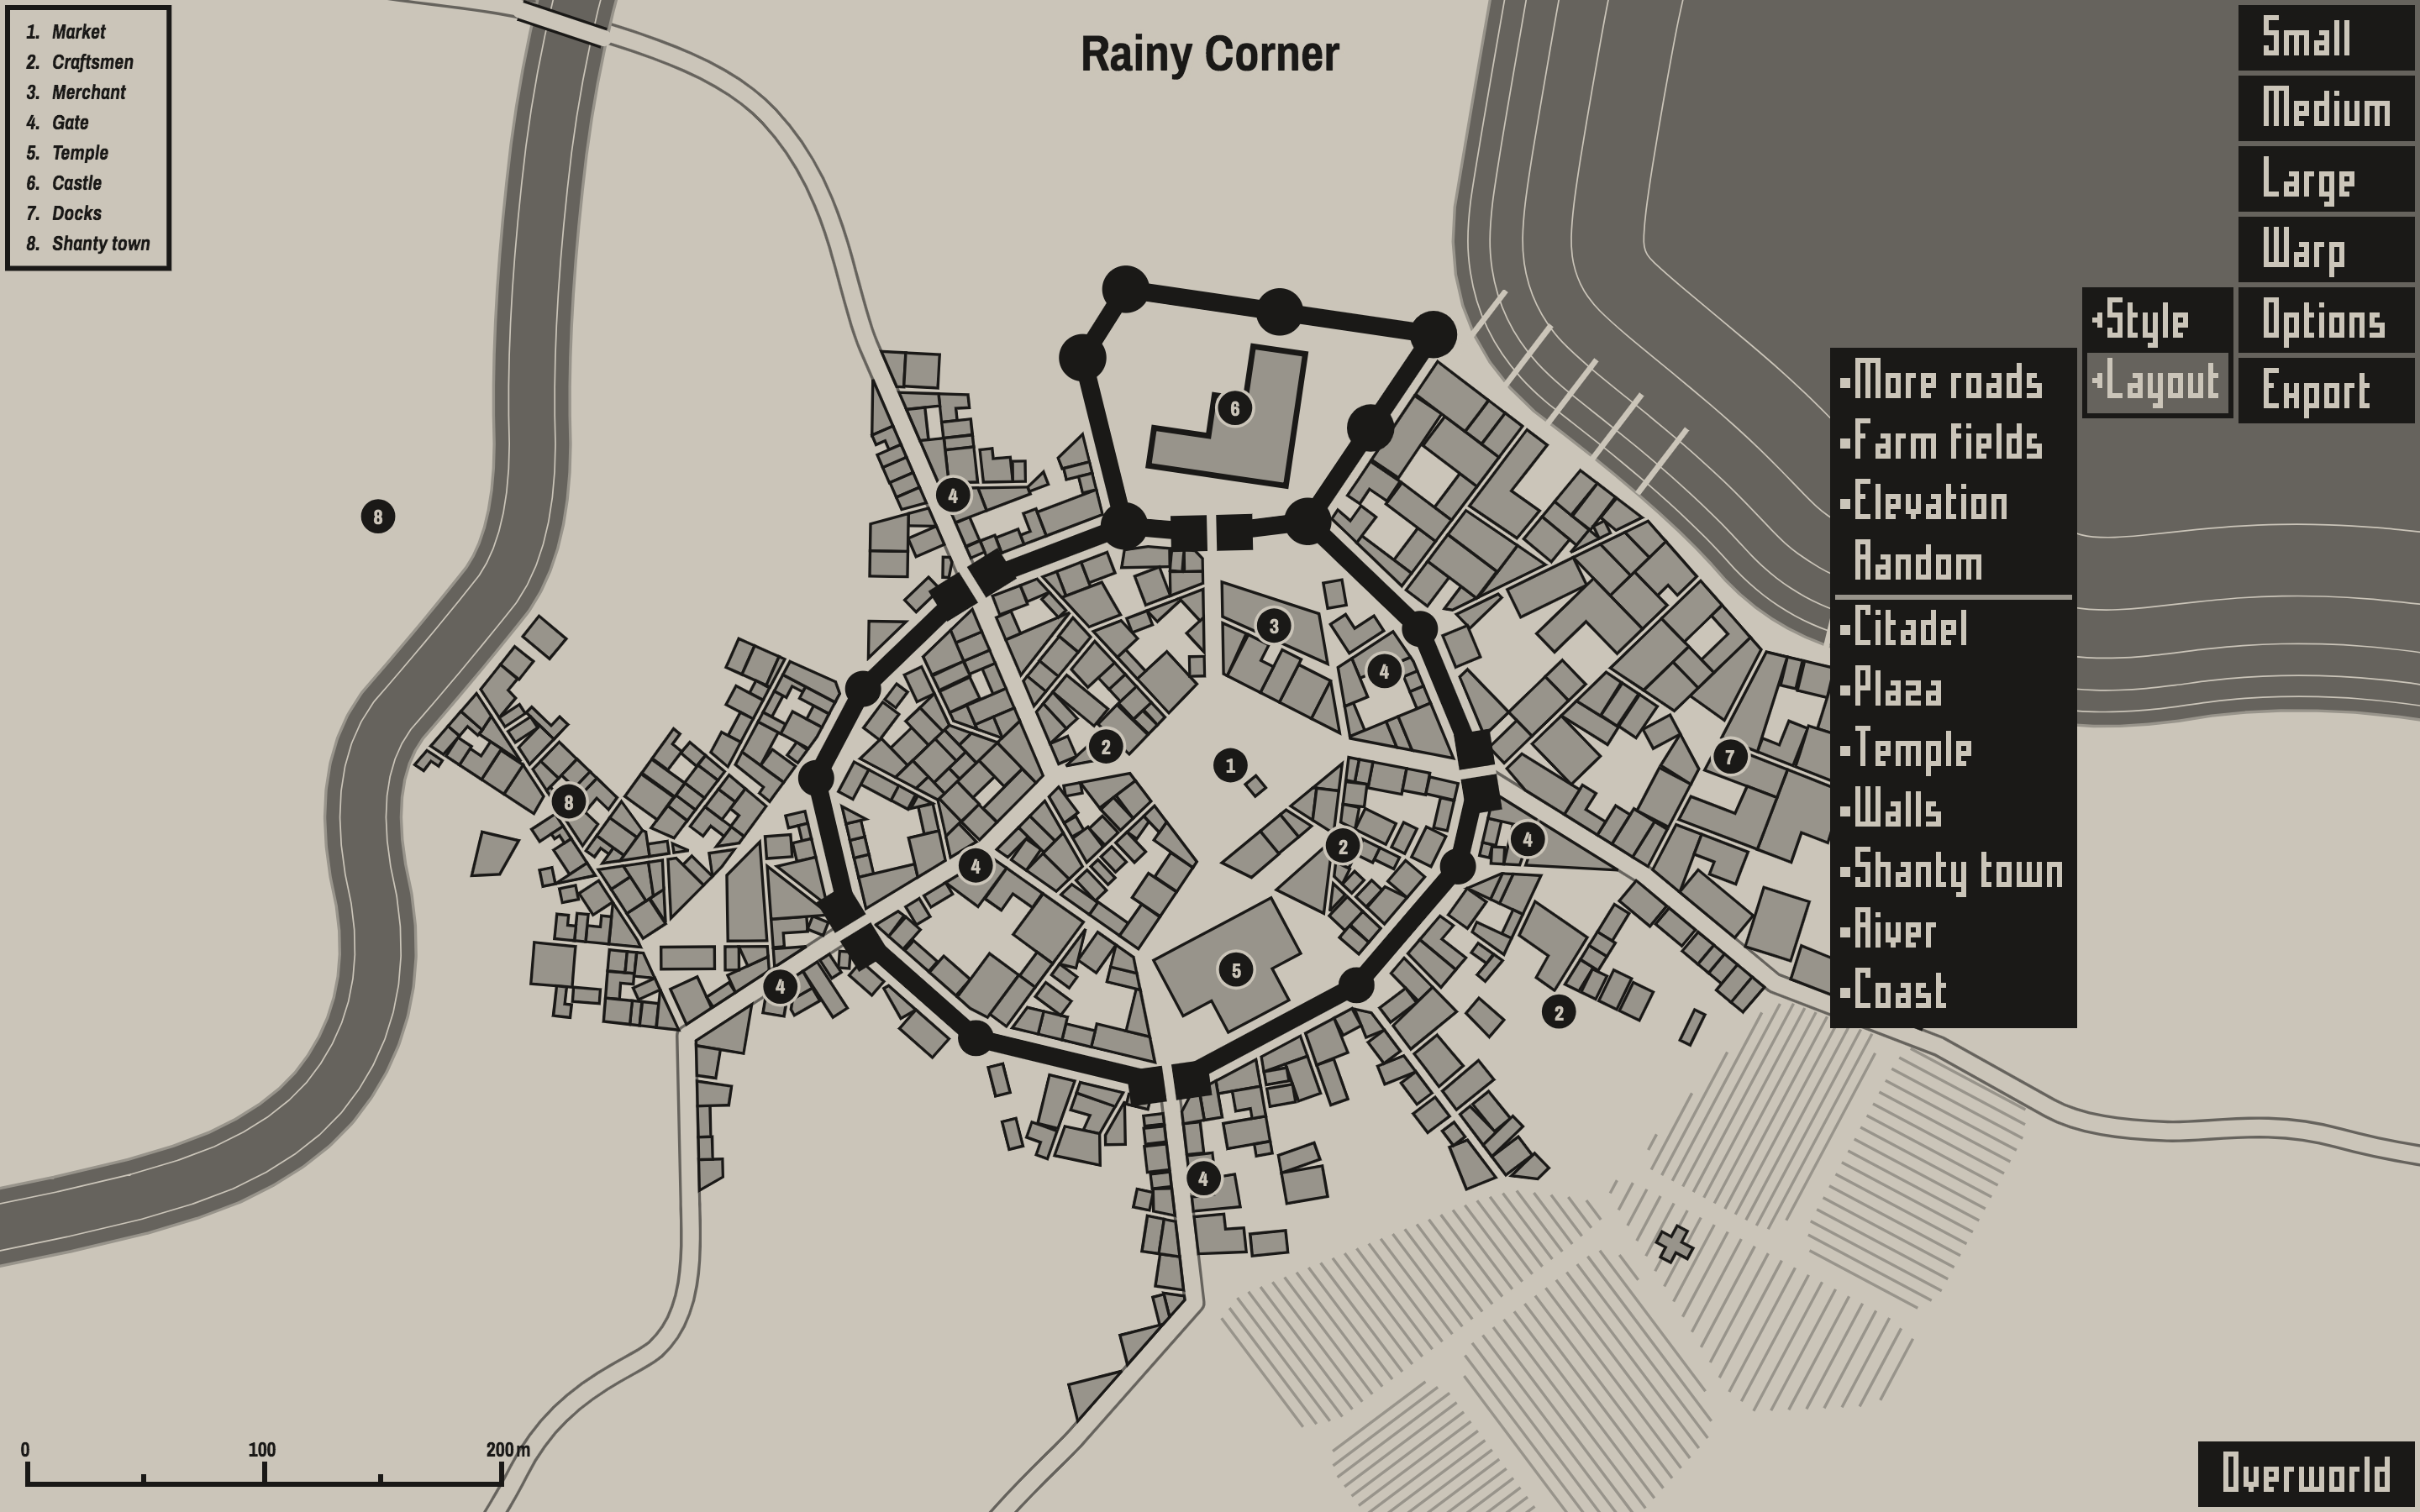
\includegraphics[width=.5\textwidth]{section01/assets/screenshot_MFCG.png}
\caption[A screenshot of Medieval Fantasy City Generator]{\label{Screenshot MFCG}A screenshot of Medieval Fantasy City Generator}
\end{figure}

The Azgaar's Fantasy Map Generator(FMG) is another similar application. Project goal is a procedurally generated map for author's Medieval Dynasty simulator. Map can be interactive, scalable, fast and plausible. There should be enough space to place at least 500 manors within 7 regions. The imagined area is about 200.000 km^2. Figure \ref{Sample Map 1} is a sample of this wonderful simulator.

\begin{figure}[htb]
\centering
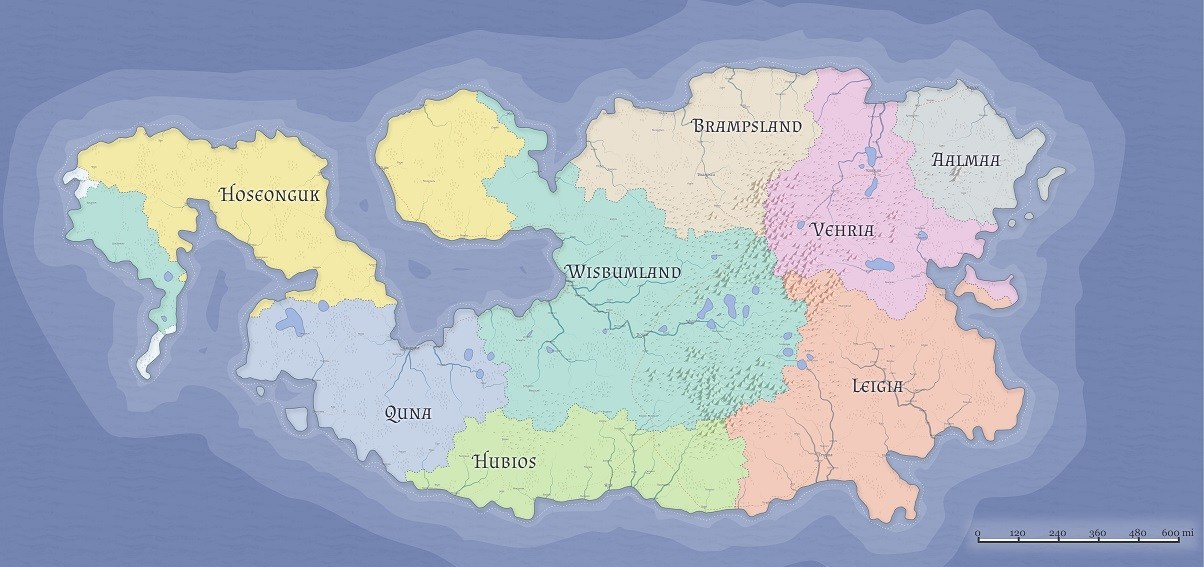
\includegraphics[width=.5\textwidth]{section01/assets/sample_map1.jpeg}
\caption[An example map of Azgaar's Fantasy Map Generator]{\label{Sample Map 1}An example map of Azgaar's Fantasy Map Generator}
\end{figure}

\subsection{Project Goal}
Our project goal is
